\section{Elektros srovė. Omo dėsnis.}

\begin{defn}[Elektros srovė]
  Tvarkingas ir kryptingas laisvų elektringų dalelių (krūvininkų)
  judėjimas.
\end{defn}

\begin{defn}[Srovės stipris]
  Skaliarinis fizikinis dydis lygus:
  \begin{align*}
    I = \frac{dq}{dt}.
  \end{align*}
  čia $dq$ – krūvio pokytis, $dt$ – laiko pokytis.
\end{defn}

\begin{defn}[Srovės tankis]
  \begin{align*}
    j = \frac{dI}{dS} \left( = \frac{q}{S} \right).
  \end{align*}
\end{defn}

Elektros srovės priežastimi negali būti Kuloninės jėgos. Reikia, kad
krūvininkus veiktų dar ir neelektrostatinės jėgos (pašalinės jėgos).

\begin{defn}[Elektros srovė metaluose]
  Tai tam tikra tvarka ir kryptimi judantys elektronai. Jie susiduria su
  apie pusiausvyros padėtį svyruojančiais elektronais ir jonais ir
  praranda dalį kinetinės energijos.
\end{defn}

\begin{defn}[Omo dėsnis diferencialinėje formoje]
  \begin{align*}
    \vec{j} = \underbrace{en\mu}_{\sigma}\vec{E},
  \end{align*}
  čia:
  \begin{itemize}
    \item $e$ – elektrono krūvis;
    \item $n$ – elektrono greitis;
    \item $\mu$ – elektrono dreifinis greitis;
    \item $\vec{E}$ – elektrinio lauko stipris;
    \item $\sigma$ – medžiagos laidumas, atvirkštinis dydis
      medžiagos varžai $\frac{1}{\rho}$.
  \end{itemize}
\end{defn}

\begin{defn}[Varža]
  \begin{align*}
    R &= \rho \cdot \frac{l}{S}; \\
    \rho &= \rho_{0} (1 + \alpha t); \\
    \alpha &= \frac{\rho - \rho_{0}}{\rho_{0} \cdot t}
  \end{align*}
  čia:
  \begin{itemize}
    \item $\rho$ – laidininko savitoji varža;
    \item $S$ – laidininko skerspjūvio plotas;
    \item $t$ – temperatūra laipsniais ${}^{o}C$;
    \item $\alpha = 4 \cdot 10^{-3} K^{-1}$ – daugumos grynųjų metalų.
  \end{itemize}
\end{defn}

% INCLUDE: Brėžinį iš Audriaus sąsiuvinio. ID=#0001

\begin{defn}[Elektrovaros jėga]
  Darbas perkeliant vienetinė teigiamą krūvį:
  \begin{equation*}
    \varepsilon = \frac{A_{\t{pašalinių}}}{q}
  \end{equation*}
  Elektrovaros jėgos vienetas yra voltas (kaip ir potencialų skirtumo
  bei įtampos).
\end{defn}

\begin{defn}[Vienas voltas]
  Vienas voltas yra toks potencialų skirtumas tarp dviejų taškų, kai
  pernešant tarp jų vieno kulono krūvį yra atliekamas vieno Džaulio
  darbas.
  \begin{align*}
    1 V = \frac{1J}{1C}
  \end{align*}
\end{defn}

\section{Elektros grandinių analizė}

Dvi Kirkofo taisyklės:
\begin{enumerate}
  \item Algebrinė suma srovių mazge yra lygi 0. (Krūvio kaupimo mazguose
    nėra.)
    \begin{align*}
      \sum ^{n} _{k=1} I_{k} = 0
    \end{align*}
  \item Išsišakojusios elektros grandinės uždarame kontūre (bet koks ciklas 
    grandinėje) įtampos kritimų kontūro dalyse algebrinė suma yra
    lygi evj algebrinei sumai visų šaltinių tame kontūre.
    \begin{align*}
      \sum _{k=1} ^{n} I_{k} R_{k} = \sum _{i=1} ^{m} E_{i}.
    \end{align*}
\end{enumerate}

\begin{figure}[H]
  \begin{center}
    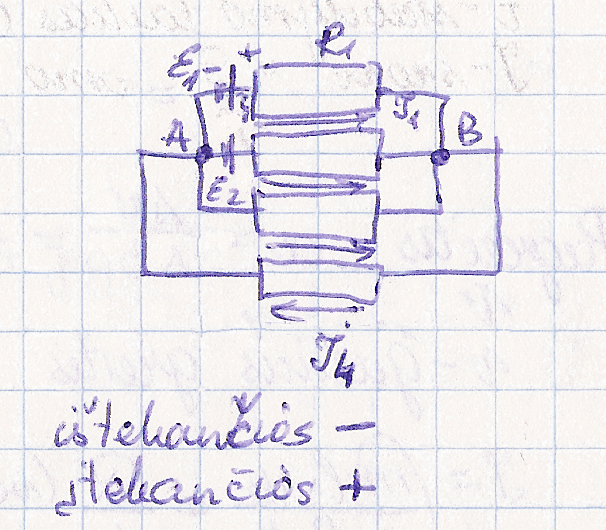
\includegraphics[height=0.5\textwidth]{images/grandine1.png}
  \end{center}
  \caption{Elektros grandinės analizė}
  \label{fig:grandine1}
\end{figure}

\begin{exmp}
  Sudarykime lygtis \ref{fig:grandine1} paveikslėlyje pateiktai grandinei.
  Sudarinėdami lygtis, ženklus nustatome tokiu būdu: jei srovės kryptis
  sutampa su ėjimo kryptimi, tada rašome $+$, priešingu atveju rašome
  $-$; jei šaltinį praeiname iš $-$ į $+$, tai rašome $+$, o jei
  iš $+$ į $-$, tada rašome $-$.

  Lygtys mazgams (kadangi iš viso yra du mazgai A ir B, tai prasmingų
  lygčių galima sudaryti $2 - 1 = 1$):
  \begin{align*}
    A: & -I_{1} - I_{2} - I_{3} + I_{4} &= 0 \\
    B: & I_{1} + I_{2} + I_{3} - I_{4} &= 0 &
      \left\{ \text{perteklinė} \right\}
  \end{align*}
  
  Lygtys kontūrams (kadangi yra trys elementarieji kontūrai, tai iš
  viso galime sudaryti 3 prasmingas lygtis):
  \begin{align*}
    +I_{1}r_{1} + I_{1}R_{1} - I_{2}R_{2} - I_{2}r_{2} &= \\
      I_{1} (r_{1} + R_{1}) - I_{2} (r_{2} + R_{2}) &=
      + E_{1} - E_{2} \\
    I_{1} \left( r_{1} + R_{1} \right) - I_{3} R_{3} &= + E_{1} \\
    I_{3} R_{3} + I_{4} R_{4} &= 0
  \end{align*}
\end{exmp}
